\chapter{Basics of Cavitation}
\label{chap:chapter1}
\section{what is cavitation?}
Cavitation occurs when the pressure is lower than the vapour pressure in a liquid medium at a given temperature. The formation of vapour cavities inside a homogenous liquid (in the absence of bubbles in the fluid stream) can occur in many different conditions.
According to the flow configuration and the physical properties of the liquid,these shows different characteristics.\\

According to Fran and Michel "Cavitation can be defined as the breakdown of a liquid medium under very low pressure".This makes cavitation relevant to the field of continuum mechanics and it applied to in which liquid medium is either statics or motion 
 In this work are focused on Hydrodynamic cavitation which is associated with water as fluid,flow over a hydrofoil and cavitation occurs when fluid changes it's liquid phase to vapour phase well below the vapour pressure.This changes occurs approximately 
 at constant temperature.The vapour bubble are consider to be void space,a cavity and a region  of the fluid in which vapour exists are called cavities.\\
\section{Tension in Liquid}
The tension of the liquid means,the liquid at 
 constant temperature could be subject to a decreasing pressure p,which fall below the saturation vapor pressure .The value of $P_V$-P is called tension,$\Delta$P and the magnitude at which the rupture
 occurs is the tensile strength of the liquid,$\Delta P_C$.The process of rupture in a liquid at roughly constant temperature is often called as cavitation.The maximum negative pressure about which water gets rupture(in the absence of dissolved gas), is ranges between$-3\cdot 10^9$ to $ -3\cdot 10^{10} $ kg/m$s^2$.
\section{Concept of Vapor Pressure} 
 The concept of vapour pressure from the classical thermodynamic view point in the phase diagram  of water from (Figure 1.1) says that the curve from the triple point Tr to the critical point C seperates the liquid 
 and vapour domains,condition of evaporation or condensation of the fluid at a pressure Pv known as vapour pressure and this is the function of temperature T.
 Cavitation in  the liquid occur by lowering the pressure at constant temperature as often happens in real fluid thus cavitation appears similar to boiling ,except driving mechanism is not the temperature but 
 change in pressure.so the path in the phase diagram is said to isothermal\\
 \begin{figure}[H]
    \centering
    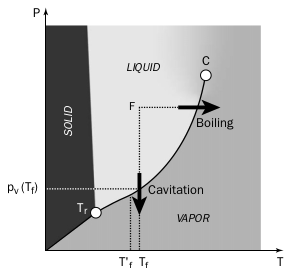
\includegraphics[scale=0.4]{phase diagram.png}
    \caption{phase diagram}
    \label{fig:fig1}
\end{figure}

 
 From theorectical view point,several steps can be distinguished during the first instants of cavitation:
  \begin{itemize}
  \item breakdown or void creation,
  \item filling of this void with vapour,
  \item eventual staturation with vapour.
  \end {itemize}
  In reality,the phases are simulaneous with the second step so instantaneous saturation of the void with vapour can be justifiably assumed.It should be kept in the mind that from phase diagram the curve Pv(T)
  is not an absolute boundary between liquid and vapour states.Deviation from this curve can also make the water not to change the phase even drop in pressure well below the vapour pressure .This was explained by ANDREWS-isotherms (Figure 1.2) in the p-v diagram,
the curves can be approximated in the liquid and vapour domains by the VANDER WAALS equation of state.The transformation from liquid to vapour along the path AM can be avoided,why because the liquid is in
metastable equilibrium and even can withstand neagative absolute pressure i.e.,tension,without any phase change special care must be take for such case while treating water for the experiment.\\
  
 
\begin{figure}[H]
    \centering
    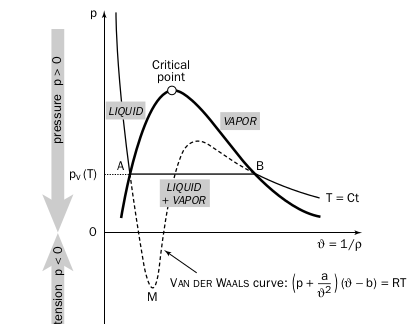
\includegraphics[scale=0.4]{ANDREW ISOTHERM.png}
    \caption{Andrews-isotherms}
    \label{fig:fig2}
\end{figure}
In conculsion,the condition that the local absolute pressure be equal to the vapour pressure at the global system temperature does not ensure that the cavitation actually occurs.This difference between the
vapour pressure and absolute local pressure at cavitation inception(first point about which phase changes starts to generates vapor bubbles)is called static delay.In some case there is also dynamic delay in 
associated with inertial phenomena with time necessary for vapor cavities to be observable.\\

\section{The Main Forms of Vapor Cavities}
Cavitation patterns of vapor structures can be divided in to three forms.These are
\begin{itemize}
\item Transient isolated bubbles:These appear in the region of low pressure well below the vapour pressure as a result rapid growth of very small air nuclei present in the liquid.They are carried along the 
stream and modify the flow.As they enter in to region of high pressure they start geting dissappear.
\item Attached or Sheet Cavities:Such cavities are often attached to the leading edge of the body.
\item Cavitating Vortices:Cavitation can appear in the low pressure core of the vortices in the turbulent wake.
\end{itemize}
Some vapour structure with short lifetime can appear on the surface of the foils or propeller blades do not fall under these three forms,eventhought they have the form of attached cavities but are 
transported similarly to traveling bubbles.This type of form was taken place in our model.\\
\section{Cavitation Regimes}
For the pratical purpose it is necessary to classifying the cavitation region.
\begin{itemize}
\item Cavitation Inception:the limiting regime between the non-cavitating condition and the cavitating flow.
\item Developed Cavitation:the where there is a extent of the cavitation zone or siginificant fall in the performance of the machines.
\end{itemize}
In our work we are mainly concerned about the extent region of cavitation zone where there will be  a high influence in unsteady cavitation shedding.The influencing situation that favorable for the 
cavitation is wall geometry which give rise to the local increment in the velocity with drop in local pressure, and shear flows due to large turbulent pressure fluctuations.\\
\section{Introduction to Nucleation}
The existence of point of weakness in the liquid due to the formation of small gas and vapor inclusions and operate at the starting points of the liquid breakdown.They are known as caviation nuclei.They are 
in few micrometers and some hundrend of micrometers.They remain spherical at this scale due to surface tension.There is two types of nucleation they are
\begin{itemize}
\item Homogeneous nucleation:when the pressure is well below the saturation pressure the liquid form temporary,microscopic voids that can constitute the nuclei,necessary for rupture and growth of bubbles.
\item Heterogeneous nucleation:nucleation might can occur at the junction of the liquid and solid boundary or due the contaminant very small sub-micron sized particles in the liquid or due to the
contaminant gas particles as micro-sized bubbles which could present in the crevices within the solid boundary or with in the suspended particles or could freely suspended in the liquid which could cause 
 weekness of the fluid  under operation.
 \end{itemize}
 Kinetic theories have also been developed to cover such heterogenous nucleation and allow to evaluate the whether the chance that this will occur in larger or smaller than the chance of homogeneous nucleation.
 Another effect has less  in contributing nucleation is cosmic radiation i.e.,collision of molecules due to high energy photon cause nucleation,but it have little chance to occur so we neglect these
 effect from this work.Most of the cases heterogeneities inside the homogeneous medium is taken in to consideration  because it is inevitable.\\
 Few things that we need to remember that,completely removing contaminated gas from the water is impossible so these effect must be taken in to consideration.So our dependence is completely depend on the
 experiment data why because including these weekness in the numerical simulation is impossible so some external parameters has to be implemented which can provide these effect .This why the reason we include non-dimensional parameter called cavitation number and cavitation inception
 in this work.\\
 \section{Homogeneous Nucleation Theory}
 Why this theory is important?
 This theory is the basic understanding of Rayleigh-Plesset equation which is a basic travelling bubble transport equation will be explained further.\\
 Consider a spherical microbubble,containing gas and vapor(heterogeneous nuclei over homogeneous nuclei) in equlibrium within the liquid at rest.The liquid can withstand negative pressure which means 
 that it is in metastable state according ANDREWS-isotherm cure(Figure 1.2).The bubble radius R which sufficiently smaller so that the hydrostatic pressure $2\rho gR$ can be neglected in comparision with 
 surface tension 2S/R.This condition requires R be smaller than the limiting value namely 2.7mm for water.This condition fulfilled in this case because the microbubble whose diameter is smaller than 0.5mm
 only are considered.The pressure can be uniform in the bulk of the surrounding fluid where there is the bubble and this microbubble is actually in spherical.The spherical shape in the bubble is mainly due
 the surface tension which state that "intermolecular forces that tend to hold the molecules together and prevent the formation of large hole".\\
 
 \begin{figure}[H]
    \centering
    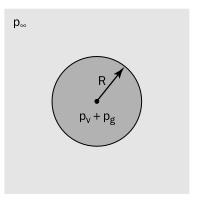
\includegraphics[scale=0.5]{bubble force equilibrium.png}
    \caption{Microbubble in liquid}
    \label{fig:fig3}
\end{figure}
The pressure equilibrium of the interface between the fluid surrounding and bubble surface is given by\\
   \begin{equation}
      P_{\infty} =P_g + P_v -\frac{2S}{R}
      \end{equation}
      ${P_\infty}$ is the surrounding bulk uniform pressure,$P_g$ gas pressure inside the bubble,$P_V$vapor pressure,S surface tension,R radius of the bubble.\\
  It is assumed that pressure change is slow enough to achive mechanical equilibrium.However the change in pressure must be in rapid enough to ensure the gas diffusion at the interface is negligible.In
  other words,the transformation is assumed to isothermal and the mass of the gas inside the bubble is constant.\\
  For the initial state,denoted by subscript 0 above equation(1.1)is written by
 \begin{equation}
 P_{{\infty}{0}} =P_{g0}+P_V-\frac{2S}{R_0}
 \end{equation}
 As the gas pressure inversly propostional to the volume in the isothermal transformation,then the equation(1.1) one can obtain
 \begin{equation}
      P_{\infty} =\frac{P_{g0}}{{[{R_0}/{R}]}^{3}} +P_v -\frac{2S}{R}
      \end{equation}
  Assuming that the critical nucleus is in thermodynamic equilibrium with its surrounding after its creation.The critical radius and critical pressure are given by comparing equation(1.1)$\&$(1.2)by assuming
  virtual transformation from initial radius to critical radius under isothermal condition with mass of gas as constant as per the above assumption.The two mechanisms considered in equation(1.1)
  \begin{itemize}
  \item the internal pressure effect which tend to increase the bubble size,to reach critical size.
  \item the surface tension effect which act in the opposite direction result in extension of minimum given by
  \end{itemize}
  \begin{equation}
  R_C = R_0 \frac {3P_{g0}}{[{\frac{2S}{R_0}}]^{1/2}}
  \end{equation}
  
  \begin{equation}
  P_C = P_V -{\frac{4S}{3R_C}}
  \end{equation}
  The mass of gas is said to constant and it is directly proportional to the $P_{g0}{{R_0}^3}$.To use the condition of constant mass of gas either use one of the doublets
   ($R_0 ,P_{\infty}$),($R_0,P_{g0}$) or preferably one of the quantities $R_c or P_c $.The stability of nucleus are given in the(Figure 1.4)in which the mechanical equilibrium of the specific nucleus 
   is stable on the branch of the curve that has negative slope.The other branch which is on right side is said to be unstable.\\
   \begin{figure}[H]
    \centering
    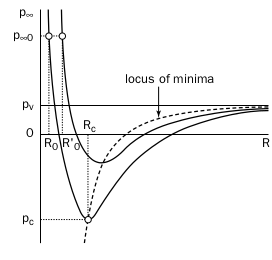
\includegraphics[scale=0.5]{stability curve.png}
    \caption{Equilibrium of a sphere nucleus}
    \label{fig:fig4}
    \end{figure}
    \section{Concept of Cavitation Number}
    The coefficient of pressure $C_{pmin}$ for an ideal fluid is depend on geometry when the effect of viscosity is included the $C_{pmin}$ is also a function of Reynolds number $R_e$.For this instance we just
    consider only the $C_{pmin}$ as a function of geometry only.
    
    \begin{equation}
    C_{px} =\frac {P_x-P_{\infty}}{{0.5 \rho {U^{2}_{\infty}}}}
    \end{equation}
   The overall pressure decreased or flow velocity increased so that the pressure at some point in the flow approaches the vapor pressure,$P_v$ of the liquid at some reference temperature $T_{\infty}$.In 
   order to relate these natural effects into a parameter,we introduced a new non-dimensional term called Cavitation number $\sigma$.The cavitation number $\sigma$ are related with the $C_{pmin}$ are 
   given below as 
   \begin{equation}
   \sigma =\frac{{P_{\infty}}-{{P_v}(T_{\infty})}}{{0.5 \rho {U^{2}_{\infty}}}}
   \end{equation}
  For sufficiently large value of $\sigma$ ($P_\infty$ sufficiently large compared with $P_v$$(T_\infty)$ or $U_\infty$ sufficiently small), single-phase liquid flow will occur.When $\sigma$ reduced 
  nucleation will first occur at some point for the corresponding value of $\sigma$ called as inception cavitation number ${\sigma}_i$. The minimum pressure point is the point about which nucleation starts 
  observable i.e, vapor bubble, for this instance, neglecting the effect of dynamic delay which deals with inertial phenomena and  as per our concern with minimum pressure point in which pressure is less than or equal to the saturated
  vapor pressure. Further reduction $\sigma$ well below ${\sigma}_i$there in an increase in the formation of bubbles. \\
  By the by $C_{pmin}$ as a geometry function the condition of non-cavitation and cavitation are stated below. From the consideration of the minimum pressure point as a first starting point for the nucleation we 
  relate that point to ${\sigma}_i$ as 
  \begin{equation}
  {{\sigma}_i} =-C_{pmin}
  \end{equation}
  From the Figure(1.5),for $\sigma >$ $-C_{pmin}$ the pressure along the entire trajectory is greater than vapor pressure $P_V$ and still non-cavitating condition is respected.For $\sigma =$ $-C_{pmin}$,the nucleus encounters $P=P_V$only for infinitesimal moment where observable of nucleus is limited
  or might not be observed.For $\sigma <$ $C_{pmin}$,the nucleus experience $P<P_V$for the finite time where it is observable and travel along the streamline.\\
  \begin{figure}[H]
    \centering
    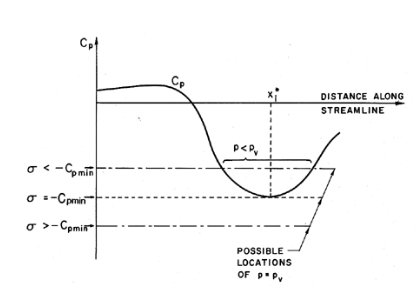
\includegraphics[scale=0.5]{pressure distribution for cp.png}
    \caption{Schematic of pressure distribution on a streamline}
    \label{fig:fig5}
\end{figure}

  In so far as free stream nucleus (heterogeneous nuclei) are concerned two main factors that cause ${\sigma}_i$ be different from $C_{pmin}$.
  First nucleation may not occur at $P=P_v$.In a degassed liquid,nucleation requires positive tension $\Delta P_c$ and hence nucleation would requires the cavitation number ${{\sigma}_i} <$$C_{Pmin}$,namely the equation relating the terms like $C_{pmin}$ and tension of the fluid i.e,
  ${{\sigma}_i}=$${-C_{pmin}}-$$\frac {{\Delta}P_c}{0.5 \rho {{{U}^2}_\infty}}$.In a liquid containing great deal of contaminant gas $\Delta P_c$ could be negative so that ${\sigma}$ would be larger than ${-C_{pmin}}$under the condition $P<{P_v}-$${\Delta}P_c$.This makes the
  ${{\sigma}_i}<$${-C_{pmin}}-$$\frac {{\Delta}P_c}{0.5 \rho {{{U}^2}_\infty}}$.So these condition should respect the assumption as isothermal.If we include the temperature then ${\sigma}_i$will also
  be the function of Temperature.Finally concluded by, when there is a great deal of contaminant gas the tension of the fluid ${\Delta}P_c$ is negative which means less in tension and rupture of fluid will
  occur faster and less in metastable equilibrium. In another sense, positive tension in the case of degassed fluid provides control in cavitation. So not only the geometry but also treating fluid for the experiment 
  is also contributed for the cavitation.
  \section{Viscous effect in cavitation inception}
  Why do we need to get cavitation inception through experiments to strengthen our work?
  The best example,In real fluid, $C_{pmin}$ is not only the function of geometry but also the contribution by the viscosity. To include this effect of viscosity the $C_{pmin}$ would be the function of 
  Reynolds number,$R_e$ so the cavitation inception,${\sigma}_i$ is a dependence of Reynolds number,$R_e$.In most,  engineering applications the flow is said to be turbulence so the vortices occur not only 
  because of the inheritance of turbulence but also due to free and forced shedding of vortices. This has major consequences in the cavitation inception ${\sigma}_i$ because the pressure at the center part of the 
  vortices is lower than the mean pressure in the flow so the cavitation first occurs at the core. so ${\sigma}_i$ will changes with $R_e$.This shows how the turbulence effect ${\sigma}_i$. There are a few other effects that 
  make the ${\sigma}_i$ to be more complicated in measurement through experiment.
  \begin{itemize}
  \item Existence of tensile strength can cause reduction in ${\sigma}_i$.
  \item Residence time effects can cause a reduction in ${\sigma}_i$.
  \item Existence of contaminated gas can cause an increase in ${\sigma}_i$.
  \item Steady viscous effect due to dependence of $C_{pmin}$ on $R_e$ can cause ${\sigma}_i$ to be function of $R_e$.
  \item Turbulence effect can cause an increase in ${\sigma}_i$
  \end{itemize}
  If these effects are not included then ${\sigma}_i$ is only function of $C_{pmin}$.Some of the experiment technique which is used to measure the ${\sigma}_i$ is the device based on acoustic scattering and light
  scattering have been used to measure the number of nuclei present in the liquid. Other instruments known as cavitation susceptibility meters cause a sample of liquid to cavitate and measure the number and size of the 
  resulting microscopic bubbles. The discussion of this technique is out of the scope of this topic.
  \section{Types of Cavitation}
  \subsection{Travelling Bubble Cavitation}
  The bubble began as micron-sized nuclei in the liquid of the oncoming stream and the bubble moved with the flow free stream velocity close to the solid body.Cavitation inception was deemed to occur 
  when the bubble reaches an observable size.
  \begin{figure}[H]
    \centering
    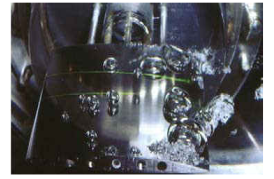
\includegraphics[scale=0.6]{travellingbubble.png}
    \caption{Travelling bubble on the surface of an hydrofoil}
    \label{fig:fig6}
\end{figure}
\subsection{Vortex Cavitation}
This type cavitation comes under large-scale cavitation structures. Cavitation inception often occurs at the core of the vortices when the core pressure is well below the mean flow pressure.
For high $R_e$ the vortices in a turbulent mixing layer or wake will also cavitate. This type is often seen in the tip vortices in the ship's propellers or pump impellers.
The three-dimensional shedding of vortices from a finite aspect ratio foil often leads to the formation and propagation 
of a ring vortex with a vapor core. In our work, there is only two-dimensional analysis so three-dimensional shedding is excluded.
\begin{figure}[H]
 \centering
 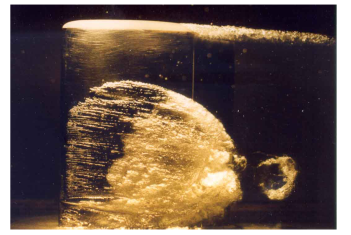
\includegraphics[scale=0.5]{Vortexcavitation.png}
 \caption{ring vortex on the surface of an hydrofoil}
  \label{fig:fig8}
\end{figure}
\subsection{Cloud Cavitation}
This is another class of large-scale cavitation. The periodic formation and collapse of a cloud of cavitation bubbles are observed. This was our area of interest where we simulate to generate cloud shedding.
 \begin{figure}[H]
 \centering
 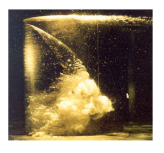
\includegraphics[scale=1]{cloudshedding.png}
 \caption{Cavitating cloud on hydrofoil}
  \label{fig:fig9}
\end{figure} 
\subsection{Shear Cavitation}
The region with high shear vorticity produced as a result coherent rational structure is formed and pressure level drop in the core of the vortices which became the potential site for the cavitation. This 
often happen in the flow separation region which is developed by the hydrofoil at very high $R_e$ and angle of attack.
\begin{figure}[H]
 \centering
 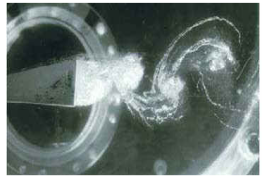
\includegraphics[scale=0.6]{shearcavitation.png}
 \caption{Shear Cavitation}
  \label{fig:fig10}
\end{figure}
\subsection{Attached/Sheet Cavitation}
These types of cavitation are often experienced in hydrofoils. In our work Attached/Sheetcavitation was been simulated through the case setup and this is the area of interest to replicate the unsteady behavior of cloud shedding.\\
\textbf{SuperCavitation}: As the cavitation parameter is decreased a small cavity attached to a hydrofoil will extend to grow longer and longer. It is because a super cavity as soon as it ceases to close the cavitation
wall but inside the liquid downstream of the cavitation. Simultaneously the lift of the foil will decrease and the drag will increases. For lower cavitation number which means low $R_e$ the supercavitation 
would experience in the foil and cavity closure will occur at the rear part. Because of lower in $R_e$ laminar separation boundary layer would experience over the hydrofoil. They showed that a well-developed 
cavity always detached downstream of laminar separation of the boundary layer. The existence of separation, which generates a relatively dead zone near to the downstream is the only way for the cavity to get attached to the wall because 
of transition to turbulence the eddy in the flow try to fix the layer near to the wall due to momentum transfer from the out side of the boundary layer to the inner layer of  flow stream and to overcome the adverse pressure effect. If there is no separation the cavity 
will be swept away by the flow. The cavity closure will be experienced on the rear part due to the cavity pressure which is lower than the surrounding pressure the balance of inertia and pressure force gives a 
curvature oriented toward the cavity.\\
\begin{figure}[H]
 \centering
 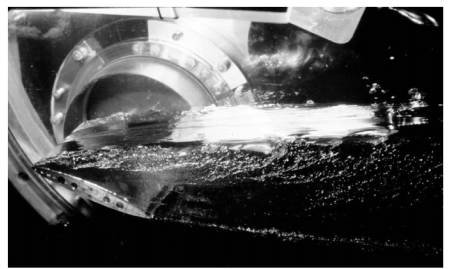
\includegraphics[scale=0.4]{supercavitation.png}
 \caption{Supercavity behind two dimensional hydrofoil}
  \label{fig:fig11}
\end{figure}

\textbf{Partial Cavitation}:This topic is the important one that is completely followed in the entire work and the condition which is represented in this topic is the real condition that was followed in the numerical
 case set up to generate the partial cavity. In partial cavitation, the attached cavity closes on the suction side of the hydrofoil. This type of cavitation has two types,

\textbf{Open attached cavity -partial type}:It is typically frothy in appearance and has periodically varying lengths, which is associated with the shedding of vapor clouds. The re-entrant jet was not observed 
in the cavity closure although recirculation flow associated with the region of separation of flow was detected and there is turbulent reattachment. The reason for the non-observation of the reentrant jet in an open cavity
because there should be a condition related to the maximum cavity thickness which was not attained in the open cavity because of low cavitation number is associated with the low angle of attack for the case of hydrofoil
which can be seen in the figure.\\
\textbf{Closed attached cavity-partial cavity}:This has a relatively stable cavity length, a clear interface, and a cavity closure that is relatively free from the bubble and completely vapor fill. This 
shows an important aspect of introducing the single-phase flow concept by considering the vapor-filled state because bubble interaction is completely removed from the above statement of the closed partial cavity 
and assuming relative velocity between these two-phase as zero means now the flow completely transfers to a single-phase flow regime. This closed partial cavitation is being adapted in our simulation for 
unsteady cloud shedding and reentrant jet observation.\\
\begin{figure}[H]
 \centering
 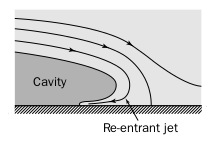
\includegraphics[scale=1]{reentantjet.png}
 \caption{closure region of partial cavity}
  \label{fig:fig11}
\end{figure}
 \textbf{Unsteady Re-entrant jet}:The reentrant jet which travels from the upstream carrying small quantity of liquid inside the cavity and the outer region reattached by turbulent reattachement.The unsteady 
 reentrant jet cavity is largely vapor-filled the cavity interface is close near the suction rear side where maximum cavity length is observed
from a thin reentrant jet flow. This reentrant jet causes the cavity to periodic break-off and roll-up of a portion of the cavity when they impinge on the cavity interface. If the reentrant jet moves far upstream to cause a large portion of the cavity to 
break off the process creates large-scale cloud shedding. If they move to a smaller distance upstream before impingement on the cavity surface then the process is called small-scale cloud cavitation.
\begin{figure}[H]
 \centering
 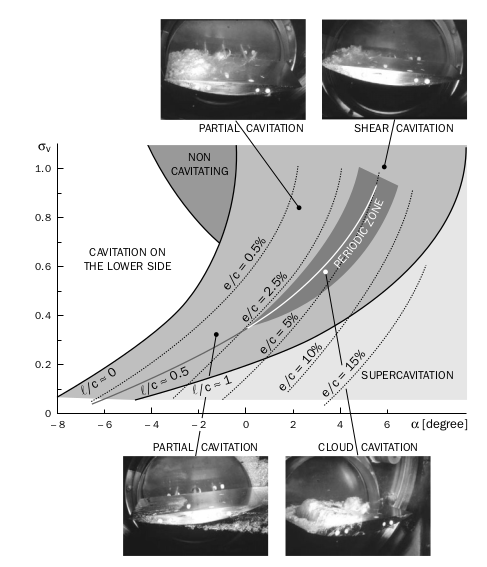
\includegraphics[scale=0.4]{partialcavitation.png}
 \caption{Main cavity patterns at $R_e =$ $2.{10}^6$ ${V_{\infty}} =10{m}/{s}$ on plano-circular hydrofoil.l is the cavity length(maximum in the case of an unsteady cavity )and e the maximum thickness of the cavity.\\}
  \label{fig:fig12}
\end{figure}
From the figure(1.12) we can see that the open cavity at low cavitation and low angle of attack where the re-entrant is not observed or weak in re-entrant flow but there is a turbulent reattachment. At the
same time in the periodic zone regime, we can see cloud shedding at a higher angle of attack and higher cavitation number along with ratio of cavitation thickness to the chord $e/c$ is minimum and 
the ratio of the length of the cavity to chord $l/c$ is around half the length of the chord act as a maximum $l/c$ i.e, a peculiar instability develops for partial cavities of medium length. On the other hand, it was limited 
by the minimum cavity thickness. Such limits suggest that a minimum value of cavity thickness is required for the periodic regime to develop. This also shows that cavity thickness must 
be larger than the reentrant jet thickness for this instability to occur along with another condition like the periodic regime is bounded by the maximum value of the cavity length which indicates that instability 
should not occur for very long cavities. This condition also holds for the reentrant jet which requires a minimum threshold value of the adverse pressure gradient to gain the impulse. Finally concluding this topic by, 
there must be minimum cavity thickness to chord ratio simultaneously maximum length of the cavity to chord ratio is required to obtain partial periodic cavity shedding along with energetic re-entrant jet. These conditions are 
well respected in this work for such kind of observatio.\\
\section{Main Effect of Cavitation in Hydraulics Performance}
\begin{itemize}
\item drop down the performance of the hydraulics system like reduction in lift and increase in drag of the foil, fall turbomachinery efficiency, reduced capacity to evacuate water in spillways, energy 
dissipation, etc.
\item the appearance of additional forces in the solid structures.
\item production of noise and vibration,
\item wall erosion when the bubble gets extruded between the fluid and solid surface caused the solid surface to erode and this effect  acts like a creep where it reduces the useful lifetime of the machine.
\end{itemize}

\chapter{Theoretical Formulation}
\label{chap:chapter2}





  
  
  
  
  
  
  
  
  
  
  
  
  
  
  
  
  
  
  
  
  
  
  
  
  
  
  
  
  
  
  
  
  
  
  
  
  
  
  
  
	        
 




















































 
